\section{Thin-film Airy formula}

The fourth example pushes the benchmark from two to three media by placing
a single finite film between two half-spaces and comparing the TMM against
the closed-form Airy formula at normal incidence. Three configurations are
run in parallel, sweeping the wavelength from \SI{300}{\nano\metre} to
\SI{1000}{\nano\metre}:

\begin{itemize}
  \setlength{\itemsep}{0.2em}
  \item Case (a): air ($n_0 = 1$) / lossless film ($n_1 = 2.0$) / glass ($n_2 = 1.5$), film thickness $d = \SI{100}{\nano\metre}$;
  \item Case (b): air / absorbing film ($n_1 = 3.0 + 0.05\,\ii$) / glass, $d = \SI{500}{\nano\metre}$;
  \item Case (c): air / absorbing film ($n_1 = 3.0 + 0.05\,\ii$) / absorbing substrate ($n_2 = 3.11 + 4.89\,\ii$), $d = \SI{500}{\nano\metre}$.
\end{itemize}

Case (a) is purely interferometric, case (b) adds weak absorption in the
film, and case (c) makes both the film and the substrate complex, which
tests the branch-cut convention of both the film wavenumber and the
substrate Fresnel coefficient simultaneously. The analytic reference is
the Airy formula for a single film,
\begin{equation}
  r = \frac{r_{01} + r_{12}\,e^{2\ii\beta}}{1 + r_{01}\,r_{12}\,e^{2\ii\beta}},\qquad \beta = \frac{2\pi n_1 d}{\lambda}\cos\theta_1, \label{eq:airy-r}
\end{equation}
with $r_{jk}$ the single-interface amplitudes
of~\eqref{eq:fresnel-rs}--\eqref{eq:fresnel-rp}. The positive sign in
$e^{+2\ii\beta}$ is dictated by the $e^{-\ii\omega t}$ time convention and
is the sign that makes~\eqref{eq:airy-r} consistent with the Fresnel
amplitudes used by the TMM.

\begin{center}
\begin{tikzpicture}
  \fill[black!4] (0, 0) rectangle (5, 1.6);
  \fill[green!10] (0,-0.7) rectangle (5, 0);
  \fill[blue!6]  (0,-1.9) rectangle (5,-0.7);
  \draw[thick] (0,0) -- (5,0);
  \draw[thick] (0,-0.7) -- (5,-0.7);
  \node[lbl, anchor=east] at (4.9, 1.2) {$n_0$};
  \node[lbl, anchor=east] at (4.9,-0.35) {$n_1$, $d$};
  \node[lbl, anchor=east] at (4.9,-1.4) {$n_2$};
  \raysketch{1.6}{0}{f}
\end{tikzpicture}
\end{center}

\begin{figure}[!htbp]
  \centering
  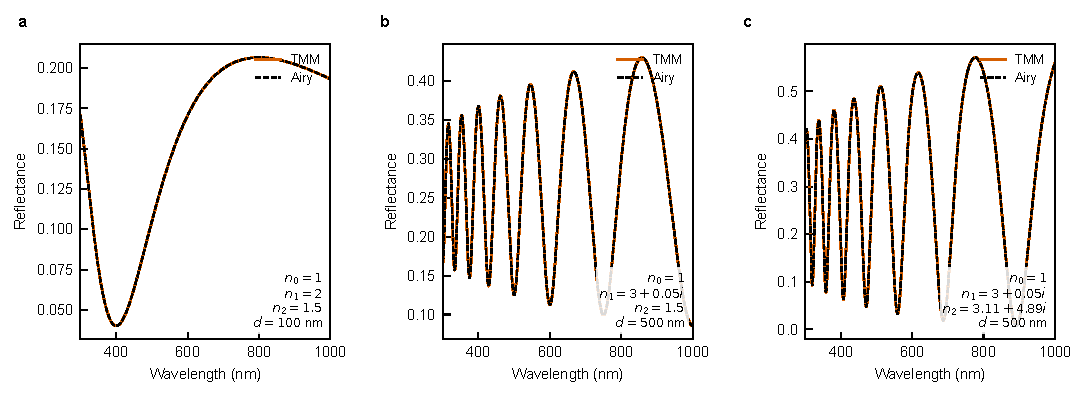
\includegraphics[width=\textwidth]{04_thin_film_airy.pdf}
  \caption{Reflectance of a single film versus wavelength for the three cases listed in the text. TMM (solid colour) overlays the Airy formula (dashed black) in each panel.}
  \label{fig:airy}
\end{figure}

Across all three cases the TMM and Airy curves coincide at
$\max|R_{\rm TMM} - R_{\rm Airy}| \approx \num{4e-15}$, independent of
whether the film or the substrate is absorbing. The residual is dominated
by the catastrophic cancellation that enters~\eqref{eq:airy-r} when the
numerator is nearly zero, and it stays at the level of floating-point
noise throughout the scan. Case (a) shows the textbook equally-spaced Airy
fringes, case (b) damps the fringe contrast towards shorter wavelengths as
the film absorption becomes significant, and case (c) adds a smooth
background from the complex substrate Fresnel coefficient on which the
attenuated fringes ride.


